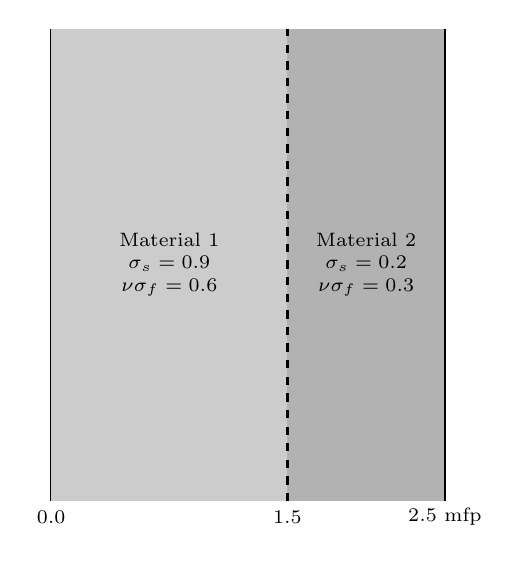
\begin{tikzpicture}[text centered]
    \begin{scope}[thick,font=\scriptsize]

    \draw [-] (-2.5,-3) -- (-2.5,3) {};
    \draw [-] (0.5,-3) -- (0.5,3) {};
    
    \draw node at (-2.5,-3.2) {$0.0$};
    \draw node at (2.5,-3.2) {$2.5$ mfp};
        \draw node at (0.5,-3.2) {$1.5$};
    
    \fill[fill=black!20] (-2.5,-3) rectangle (0.5,3);
    \fill[fill=black!30] (0.5,-3) rectangle (2.5,3);
    
    \draw [dashed] (0.5,-3) -- (0.5,3) {};
    \draw (2.5,-3) -- (2.5,3) {};
    
    \draw node [align=center] at (-1.0,0) {Material 1 \\ $\sigma_{s} = 0.9$ \\ $\nu \sigma_{f} = 0.6$};
    \draw node [align=center] at (1.5,0) {Material 2 \\ $\sigma_{s} = 0.2$ \\ $\nu \sigma_{f} = 0.3$};


    \end{scope}
\end{tikzpicture}